\chapter{Lab mmap:内存映射实验}
\begin{introduction}
    \item 实现 mmap 内存映射系统调用
    \item 再次俯瞰 xv6
\end{introduction}

虽然在现代的 Linux 操作系统中,由于新的机制的引入, mmap 系统调用已经成为 glibc 在很多情形下的备选方案,但这并不影响 mmap 作为经典的 Unix 系统调用的地位。为 xv6 实现 mmap 的过程会涉及修改操作系统的几乎每个部分,故而作为压轴实验供我们把玩。

\section{实现 mmap 内存映射系统调用}

真正的 mmap 为用户程序提供了精细化操作它们地址空间的手段,包括但不限于:共享进程间的地址空间,将文件映射到地址空间,用户处理缺页错误等功能。我们需要为 xv6 添加的 mmap 只需要实现将文件映射到地址空间的功能,其接受的参数如下:
\begin{lstlisting}[language=C]
void *mmap(void *addr, size_t length, int prot, int flags,
    int fd, off_t offset);
\end{lstlisting}

此外,另有一个用于取消 mmap 映射的系统调用 \lstinline{munmap(addr, length)} ,除了移除映射外,其根据实际情况可能需要将映射的文件写回。

xv6 实验和往常一样,为我们提供了用户态测评程序 \lstinline{mmaptest} 。在该测评程序中, addr 和 offset 总是为 0 ,意味着内核可以自由选择映射的地址,并总是从文件开头开始映射;若映射失败,则返回 \lstinline{0xffffffffffffffff} 。我们只需实现 \lstinline{mmaptest} 中用到的功能。

首先照例在 Makefile 中添加用户态测评程序 \lstinline{mmaptest} ,然后添加空的 \lstinline{mmap} 和 \lstinline{munmap} ,使得编译通过:
\begin{lstlisting}[language=C]
    Makefile:
    ==============================
    UPROGS=\
    ......
    	$U/_mmaptest\
    ......
    ==============================
    
    kernel/syscall.h
    ==============================
    ......
    #define SYS_mmap   22
    #define SYS_munmap 23
    ==============================
    
    kernel/syscall.c
    ==============================
    ......
    extern uint64 sys_mmap(void);
    extern uint64 sys_munmap(void);
    ......
    static uint64 (*syscalls[])(void) = {
    ......
    [SYS_mmap]    sys_mmap,
    [SYS_munmap]  sys_munmap,
    };
    ......
    ==============================
    
    kernel/sysproc.c
    ==============================
    ......
    void *sys_mmap(void)
    {
      return (void *)-1;
    }
    
    int sys_munmap(void)
    {
      return -1;
    }
    ......
    ==============================
    
    user/user.h
    ==============================
    ......
    void *mmap(void *, int, int, int, int, int);
    int munmap(void *, int);
    ......
    ==============================
    
    user/usys.pl
    ==============================
    ......
    entry("mmap");
    entry("munmap");
    ......
    ==============================
\end{lstlisting}

此时执行 \lstinline{make} ,应当能够编译通过。按照 xv6 实验手册的提示,在 \lstinline{proc.h} 中加入 VMA 数据结构的定义,并给进程控制块中加入 VMA 指针:
\begin{lstlisting}[language=C]
#define NVMA 16
#define VMA_START (MAXVA >> 1)

struct vma {
  uint64 start;
  uint64 end;
  uint64 length; // 0 -> not used
  uint64 off;

  int perm;
  int flags;
  struct file *file;
  struct vma *next;

  struct spinlock lock;
};

// Per-process state
struct proc {
......
  struct vma *vma;             // VMA item
};
\end{lstlisting}

为了避免于堆和栈冲突,这里我们决定将内存映射开始于最大地址的一半处。由于后续需要多次对 VMA 进行分配,故而将其封装为一个函数会更加方便,\lstinline{proc.c} 中加入:
\begin{lstlisting}[language=C]
......
// VMA list
struct vma vma_list[NVMA];

struct vma* vma_alloc() 
{
  for(int i = 0; i < NVMA; i++)
  {
    acquire(&vma_list[i].lock);
    if (vma_list[i].length == 0)
    {
      return &vma_list[i];
    } else 
    {
      release(&vma_list[i].lock);
    }
  }
  panic("no free vma");
}
......
\end{lstlisting}

然后,根据实验手册的提示,我们无需真正在 \lstinline{sys_mmap} 中完成内存映射,而是通过一个惰性机制,在出现缺页异常时再进行映射,故而我们在 \lstinline{sys_mmap} 中只需完成对 VMA 的设置:
\begin{lstlisting}[language=C]
#include "types.h"
#include "param.h"
#include "date.h"
#include "spinlock.h"
#include "sleeplock.h"
#include "fs.h"
#include "memlayout.h"
#include "riscv.h"
#include "defs.h"
#include "proc.h"
#include "fcntl.h"
#include "file.h"
......
extern struct vma *vma_alloc();
void *sys_mmap(void)
{
  uint64 addr;
  struct proc *p = myproc();
  int length, prot, flags, fd, offset;

  if (argaddr(0, &addr) < 0)
    return (void *)-1;
  if (argint(1, &length) < 0)
    return (void *)-1;
  if (argint(2, &prot) < 0)
    return (void *)-1;
  if (argint(3, &flags) < 0)
    return (void *)-1;
  if (argint(4, &fd) < 0)
    return (void *)-1;
  if (argint(5, &offset) < 0)
    return (void *)-1;
  if (addr != 0)
    addr = 0;
  if (offset != 0)
    offset = 0;

  struct file *f = p->ofile[fd];

  // Check flags
  int pte_flag = PTE_U;
  if (prot & PROT_READ)
  {
    if (!f->readable)
      return (void *)-1;
    pte_flag |= PTE_R;
  }
  if (prot & PROT_WRITE)
  {
    if (!f->writable && !(flags & MAP_PRIVATE))
      return (void *)-1;
    pte_flag |= PTE_W;
  }

  // Setting up vma
  struct vma *v = vma_alloc();
  v->perm = pte_flag;
  v->length = length;
  v->off = offset;
  v->file = myproc()->ofile[fd];
  v->flags = flags;
  filedup(f);
  struct vma *pv = p->vma;
  if (pv == 0)
  {
    v->start = VMA_START;
    v->end = length + v->start;
    p->vma = v;
  }
  else
  {
    while (pv->next)
      pv = pv->next;
    v->start = PGROUNDUP(pv->end);
    v->end = v->start + length;
    pv->next = v;
    v->next = 0;
  }
  addr = v->start;
  release(&v->lock);
  return (void *)(addr);
}
......
\end{lstlisting}

为了在 \lstinline{usertrap} 中处理 mmap 造成的缺页异常,我们首先编写相关的中断处理过程 \lstinline{mmap_alloc} :
\begin{lstlisting}[language=C]
#include "types.h"
#include "param.h"
#include "memlayout.h"
#include "riscv.h"
#include "spinlock.h"
#include "sleeplock.h"
#include "proc.h"
#include "defs.h"
#include "fs.h"
#include "file.h"
......
int mmap_alloc(uint64 va, int scause)
{
  struct proc *p = myproc();
  struct vma* v = p->vma;

  while(v != 0)
  {
    if (va >= v->start && va < v->end)
    {
      break;
    }
    v = v->next;
  }

  if (v == 0) 
    return -1; 
  if (scause == 13 && !(v->perm & PTE_R)) 
    return -1; 
  if (scause == 15 && !(v->perm & PTE_W)) 
    return -1;
  
  // load from file
  va = PGROUNDDOWN(va);
  char* mmem = kalloc();
  if (mmem == 0) 
    return -1;
  memset(mmem, 0, PGSIZE);

  if (mappages(p->pagetable, va, PGSIZE, (uint64)mmem, v->perm) != 0)
  {
    kfree(mmem);
    return -1;
  }

  struct file *f = v->file;
  ilock(f->ip);
  readi(f->ip, 0, (uint64)mmem, v->off + va - v->start, PGSIZE);
  iunlock(f->ip);
  return 0;
}
......
\end{lstlisting}

在 \lstinline{usertrap} 中调用 \lstinline{mmap_alloc} :
\begin{lstlisting}[language=C]
void
usertrap(void)
{
......
  } else if((r_scause() == 13) || (r_scause() == 15)){  // page fault
    if (mmap_alloc(r_stval(), r_scause()) != 0) 
    {
      printf("mmap: page fault\n");
      p->killed = 1;
    }
  } else {

}
\end{lstlisting}

此时, mmap 的前半部分基本完成,接下来需要实现 \lstinline{munmap} 。思路与之前类似,除了操作 VMA 外,一个难点在于写回。为此我们先实现写回的函数:
\begin{lstlisting}[language=C]
void write_back(struct vma *v, uint64 addr, int n)
{
  // no need to writeback
  if (!(v->perm & PTE_W) || (v->flags & MAP_PRIVATE))
    return;
  if ((addr % PGSIZE) != 0)
    panic("unmap: not aligned");
  struct file *f = v->file;
  int max = ((MAXOPBLOCKS - 1 - 1 - 2) / 2) * BSIZE;
  int i = 0;
  while (i < n)
  {
    int k = n - i;
    if (k > max)
      k = max;
    begin_op();
    ilock(f->ip);
    int wcnt = writei(f->ip, 1, addr + i, v->off + v->start - addr + i, k);
    iunlock(f->ip);
    end_op();
    i += wcnt;
  }
}
\end{lstlisting}

然后实现 \lstinline{sys_munmap} ,根据 xv6 的要求,只需分在头尾释放两种不同的情况,中间释放的部分无需考虑:
\begin{lstlisting}[language=C]
int sys_munmap(void)
{
  uint64 addr;
  int length;
  if (argaddr(0, &addr) < 0)
    return -1;
  if (argint(1, &length) < 0)
    return -1;
  struct proc *p = myproc();
  struct vma *v = p->vma;
  struct vma *pre = 0;
  while (v != 0)
  {
    if (addr >= v->start && addr < v->end)
      break;
    pre = v;
    v = v->next;
  }
  // not mapped
  if (v == 0)
    return -1;
  if (addr != v->start && addr + length != v->end)
    panic("munmap: middle of vma");
  if (addr == v->start)
  {
    write_back(v, addr, length);
    uvmunmap(p->pagetable, addr, length / PGSIZE, 1);
    if (length == v->length)
    {
      // free all
      fileclose(v->file);
      if (pre == 0)
      {
        p->vma = v->next;
      }
      else
      {
        pre->next = v->next;
        v->next = 0;
      }
      acquire(&v->lock);
      v->length = 0;
      release(&v->lock);
    }
    else
    {
      // head
      v->start -= length;
      v->off += length;
      v->length -= length;
    }
  }
  else
  {
    // tail
    v->length -= length;
    v->end -= length;
  }
  return 0;
}
\end{lstlisting}

至此, mmap 整体上就算完成了,但是仍有两个细节需要注意:一是 fork 时需要将父进程的 VMA 复制给子进程,二是进程退出时也需要写回所有内容。首先处理 fork :
\begin{lstlisting}[language=C]
int fork(void)
{
......
  acquire(&np->lock);
  np->state = RUNNABLE;
  np->vma = 0;
  struct vma *pvma = p->vma;
  struct vma *pre = 0;
  while (pvma)
  {
    struct vma *nvma = vma_alloc();
    nvma->start = pvma->start;
    nvma->end = pvma->end;
    nvma->off = pvma->off;
    nvma->length = pvma->length;
    nvma->perm = pvma->perm;
    nvma->flags = pvma->flags;
    nvma->file = pvma->file;
    filedup(nvma->file);
    nvma->next = 0;
    if (pre == 0)
    {
      np->vma = nvma;
    }
    else
    {
      pre->next = nvma;
    }
    pre = nvma;
    release(&nvma->lock);
    pvma = pvma->next;
  }
  release(&np->lock);

  return pid;
}
\end{lstlisting}

再处理 exit 系统调用:
\begin{lstlisting}[language=C]
extern void write_back(struct vma *v, uint64 addr, int n);
void exit(int status)
{
  struct proc *p = myproc();

  if (p == initproc)
    panic("init exiting");

  // mUnmap all vma
  struct vma *v = p->vma;
  struct vma *pvma;
  while (v)
  {
    write_back(v, v->start, v->length);
    uvmunmap(p->pagetable, v->start, PGROUNDUP(v->length) / PGSIZE, 1);
    fileclose(v->file);
    pvma = v->next;
    acquire(&v->lock);
    v->next = 0;
    v->length = 0;
    release(&v->lock);
    v = pvma;
  }

  // Close all open files.
......
}
\end{lstlisting}

至此, munmap 部分大致完成。编译并运行 xv6 ,然后运行 \lstinline{mmaptest} ,会基本通过测试,但最后一项中会得到 \lstinline{panic: uvmunmap: walk} 错误。由于 mmap 机制与原有页表的标志位含义有冲突,故此时需修改 \lstinline{vm.c} ,进行如下修改:
\begin{lstlisting}[language=C]
void
uvmunmap(pagetable_t pagetable, uint64 va, uint64 npages, int do_free)
{
  uint64 a;
  pte_t *pte;

  if((va % PGSIZE) != 0)
    panic("uvmunmap: not aligned");

  for(a = va; a < va + npages*PGSIZE; a += PGSIZE){
    if((pte = walk(pagetable, a, 0)) == 0)
      // panic("uvmunmap: walk");
      continue;
    if((*pte & PTE_V) == 0)
      // panic("uvmunmap: not mapped");
      continue;
    if(PTE_FLAGS(*pte) == PTE_V)
      panic("uvmunmap: not a leaf");
    if(do_free){
      uint64 pa = PTE2PA(*pte);
      kfree((void*)pa);
    }
    *pte = 0;
  }
}
......
void
freewalk(pagetable_t pagetable)
{
  // there are 2^9 = 512 PTEs in a page table.
  for(int i = 0; i < 512; i++){
    pte_t pte = pagetable[i];
    if((pte & PTE_V) && (pte & (PTE_R|PTE_W|PTE_X)) == 0){
      // this PTE points to a lower-level page table.
      uint64 child = PTE2PA(pte);
      freewalk((pagetable_t)child);
      pagetable[i] = 0;
    } else if(pte & PTE_V){
      // panic("freewalk: leaf");
      continue;
    }
  }
  kfree((void*)pagetable);
}
\end{lstlisting}

\begin{theorem}[为何此处忽视 panic]
    由于前文 mmap 映射的页的标志位会导致原先判断 panic 的条件被触发,从而使得在 fork 或 exit 时复制或释放页面时出现预期外的 panic ,故而此处将 panic 的语句均换为继续执行。
\end{theorem}

编译并运行 xv6 ,然后运行 \lstinline{mmaptest} ,得到类似下图的结果:
\begin{figure}[H]
  \centering
  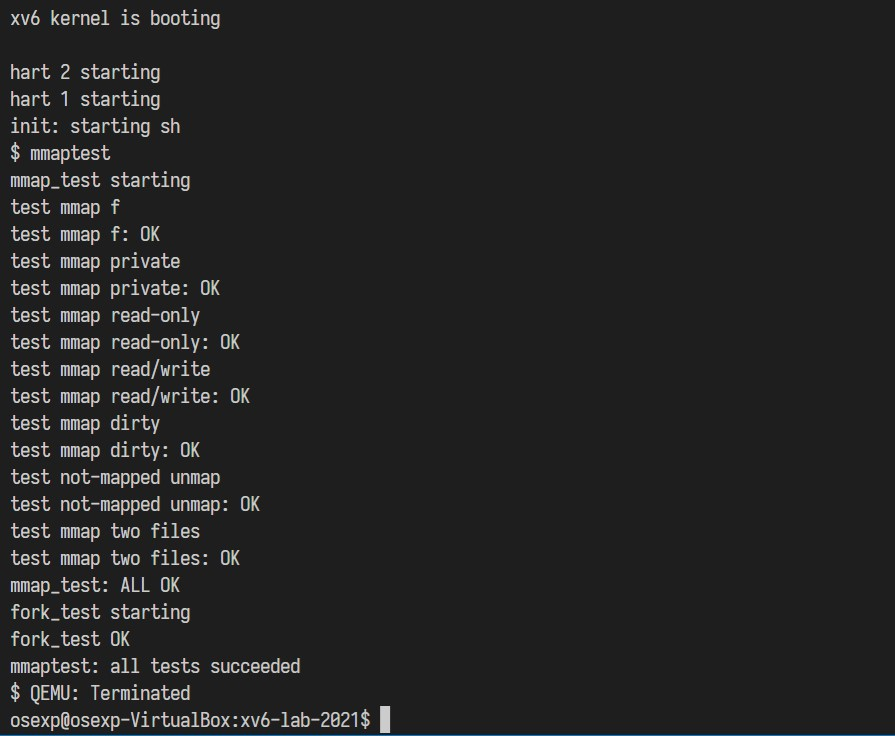
\includegraphics[width=0.6\textwidth]{mmap_mmaptest.jpg}
  \caption{ \lstinline{mmaptest} 的测试结果}
\end{figure}

测试成功通过。

\paragraph*{实验结果} 在完成 Lab mmap 中的所有实验后,根据 MIT 6.S081 的传统,需要在实验目录下创建一个名为 \lstinline{time.txt} 文本文件,其中只包含一行,为完成该实验的小时数。然后在终端中执行 \lstinline{make grade} ,即可对整个实验进行自动评分,笔者的结果如下:
\begin{figure}[H]
  \centering
  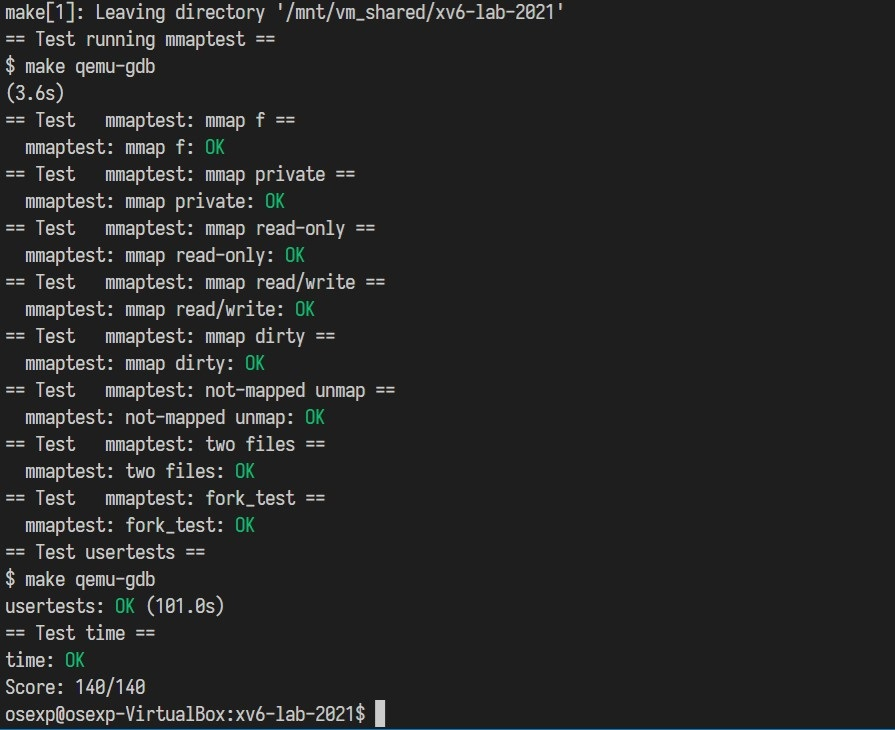
\includegraphics[width=0.6\textwidth]{mmap_grade.jpg}
  \caption{ Lab mmap 的测评结果}
\end{figure}

可见测试全部通过,得分为满分。

\section{小结:再次俯瞰 xv6}

在 mmap 实验中,我们用到了 xv6 提供的大部分机制,以它们为基础实现了较为复杂的功能。该实验作为 6.S081 提供的实验手册中的最后一次实验,起到了很好的总结作用,这里笔者也对整个 xv6 的结构做一个小结。

从用户侧来看,用户使用的主要是 \lstinline{user/user.h} ,其中包含系统调用的接口和一个 C 函数库提供的函数。系统调用接口的实现是在 \lstinline{user/usys.S} 中,而用户 C 函数库则是在 \lstinline{user/ulib.c} 中实现的。

\begin{figure}[H]
  \centering
  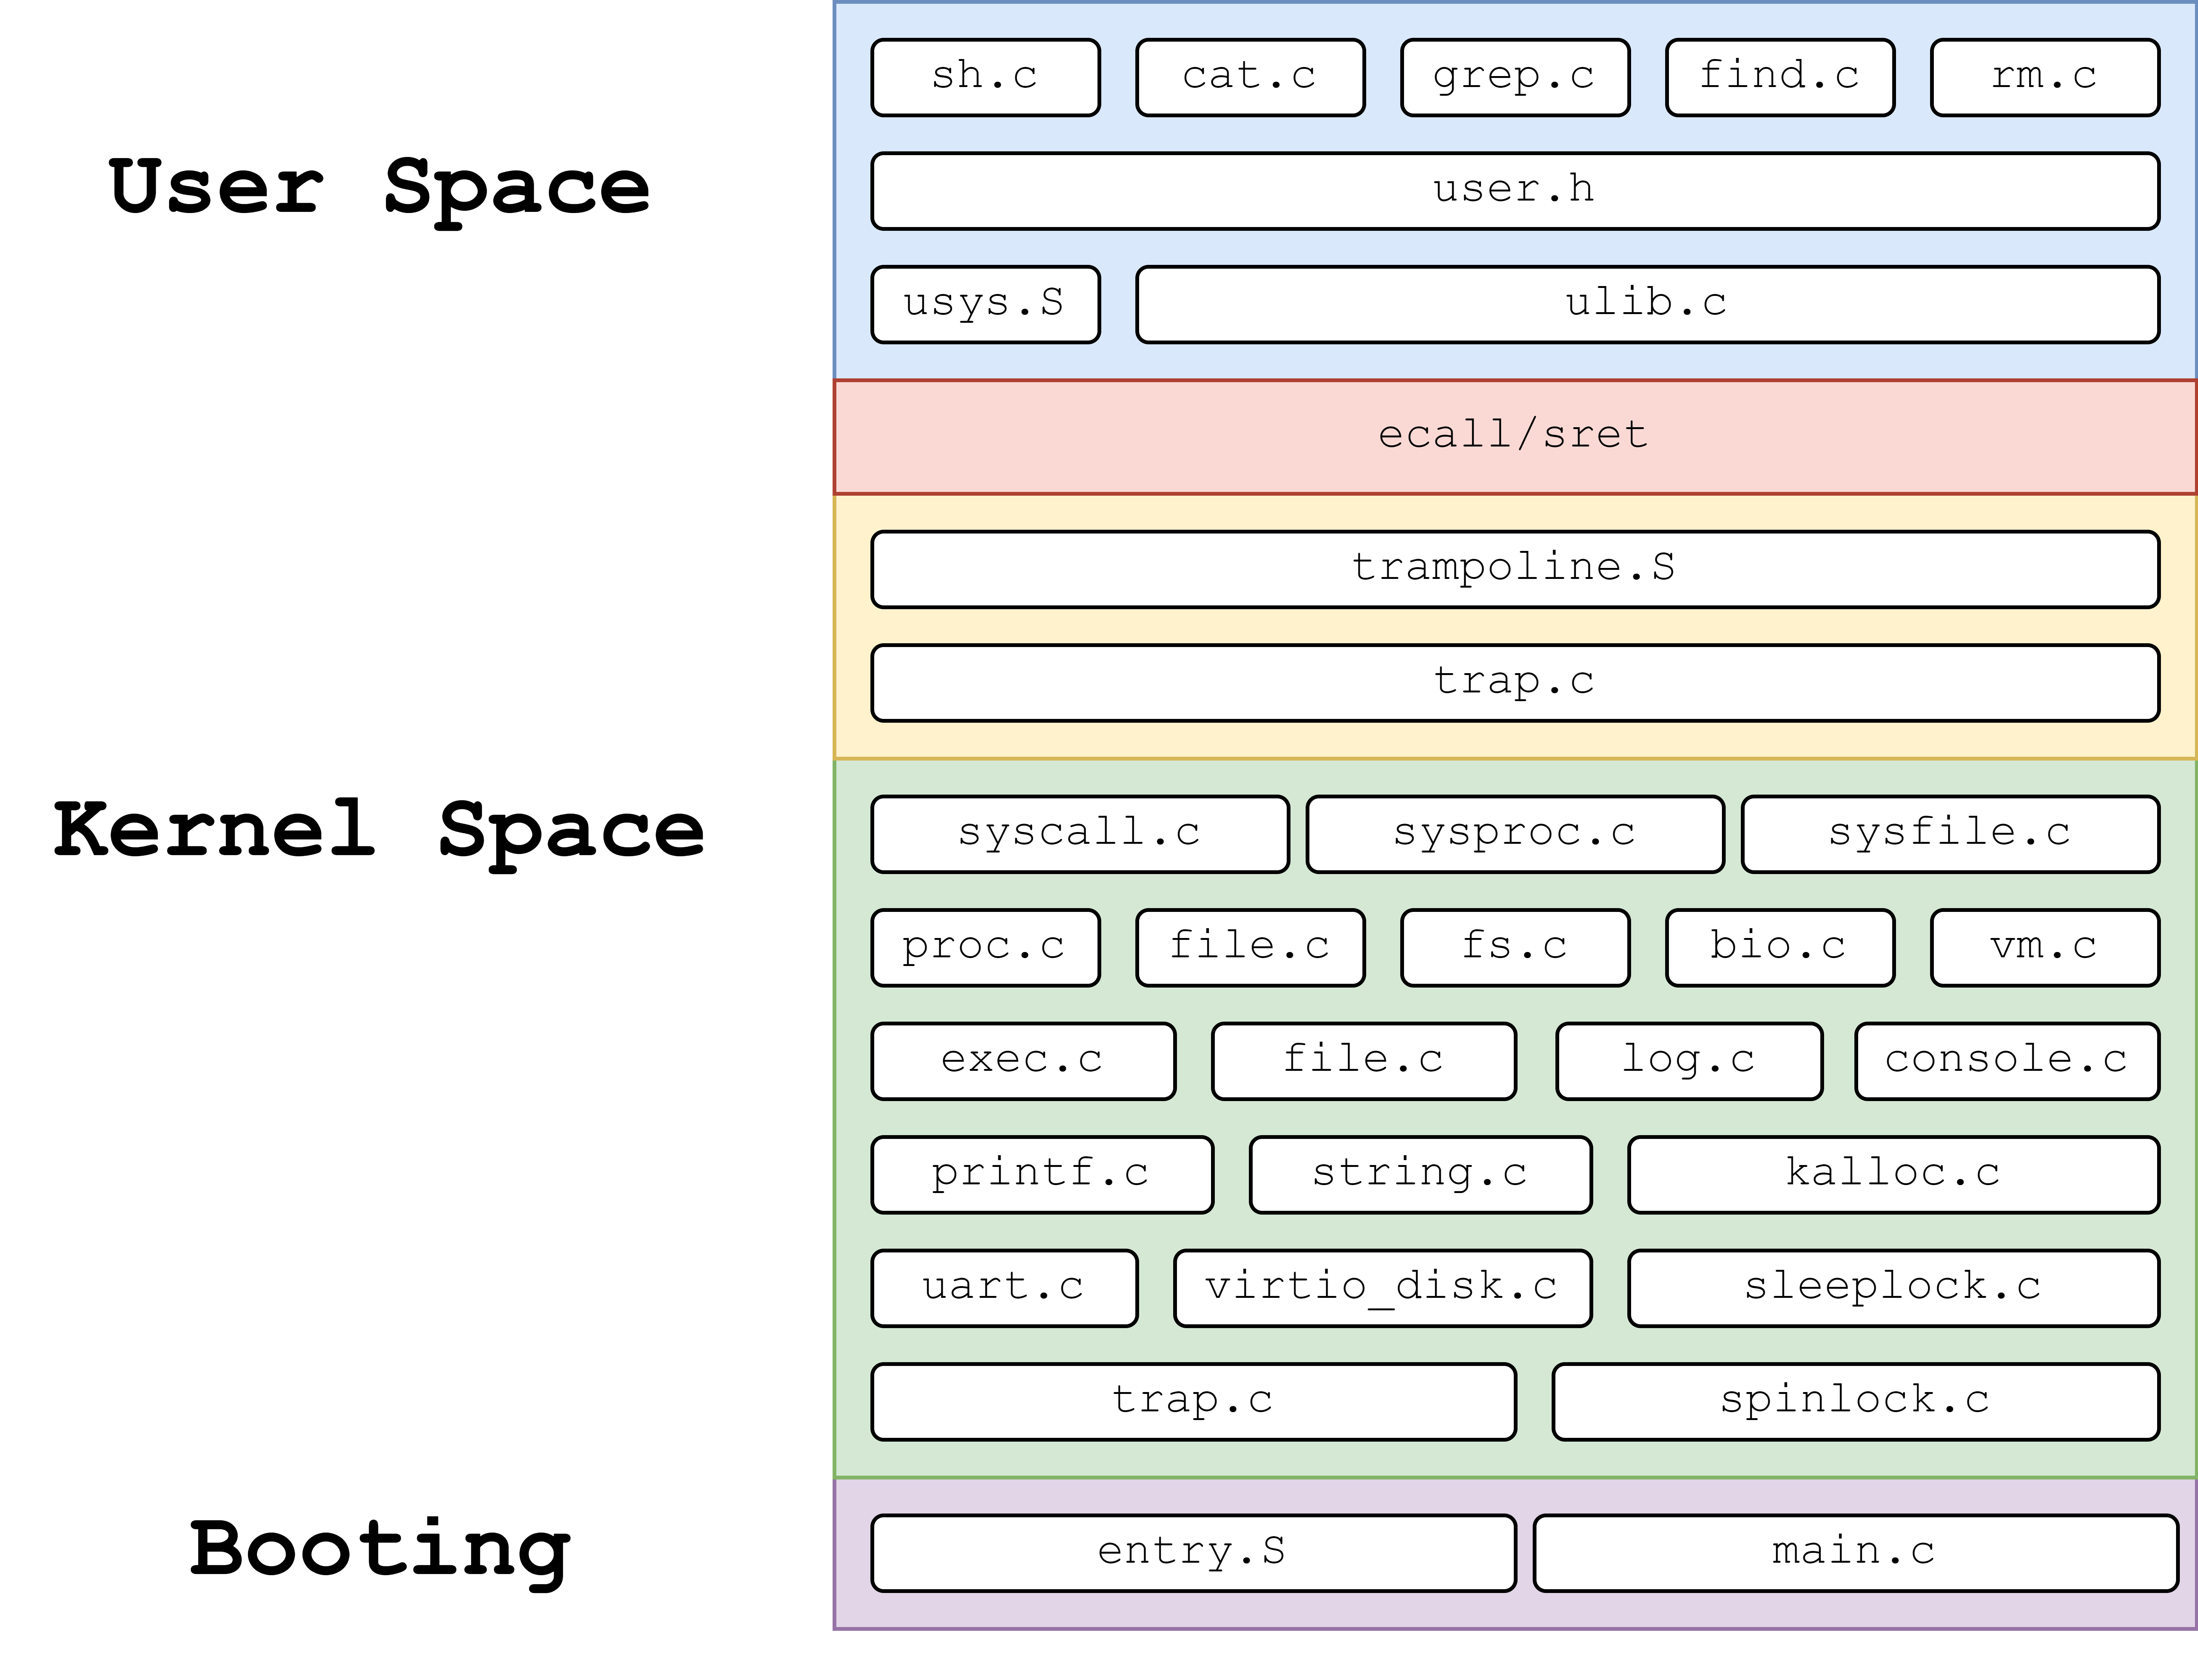
\includegraphics[width=0.8\textwidth]{xv6_arch.drawio.png}
  \caption{ xv6 结构概览 }
\end{figure}

通过 RISC-V 提供的特权指令,结合 \lstinline{trampoline.S} ,则可以完成从用户侧到内核态的跳跃; Trampoline 一词意为“蹦床”,十分形象得描述了这个过程。完成了用户侧到内核态的上下文保存与切换后,控制权移交给了 \lstinline{kernel/trap.c} 用于处理中断。内核中的诸多源文件实现了各类服务,虽然 xv6 是宏内核,但其中也有层次之分,一些较为靠近底层的功能实现和较靠近用户侧的实现是归入不同的源码文件中的:在上图中,越靠下的部分越接近硬件,诸如 \lstinline{uart.c} 等,是用于为内核中函数提供基本功能的驱动程序。还有一部分代码用于系统的初始化,这部分代码会负责从 M 态到 S 态的设置,并且为中断机制、内核内存布局进行初始化。

现代操作系统虽然也大致为分层的偏向宏内核的架构,但由于存在内核模块等机制,使得操作系统能够在运行时动态得加载或卸载功能,大大增加了操作系统的灵活性与可维护性。